\documentclass[tikz,border=5pt]{standalone}
\begin{document}
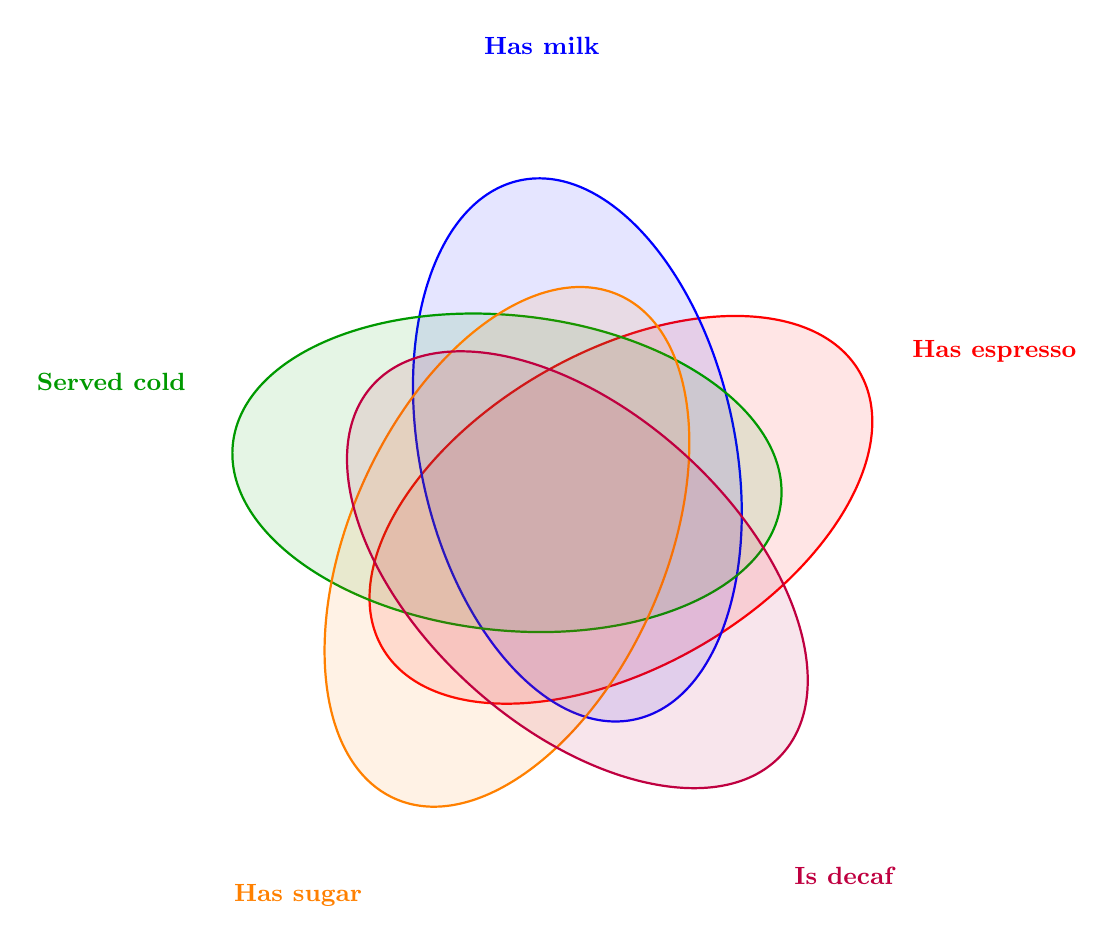
\begin{tikzpicture}
\def\names{{"Has espresso","Has milk","Served cold","Has sugar","Is decaf"}}
\foreach \i/\c in {0/red,1/blue,2/green!60!black,3/orange,4/purple}{
 \begin{scope}[rotate=72*\i]
 \draw[\c,thick,fill=\c,fill opacity=0.1,rotate around={30:(0.8,0)}] (0.8,0) ellipse (3.5cm and 2cm);
 \end{scope}
 \node[\c,font=\bfseries\small] at ({72*\i+20}:5.9) {\pgfmathparse{\names[\i]}\pgfmathresult};
}
\end{tikzpicture}
\end{document}
